\chapter*{Introduction}
At the time of writing, humanity is in the second year of the COVID-19 pandemic, at the dawn of the Omicron variant.
In its propagation, this virus has led the world in a crisis of a magnitude usually contained in History books.
All the world countries are currently facing a multifaceted crisis involving public health, social and economic issues.
However, suppose we detach ourselves from the current events.
In that case, we realize two points: (i) that crises and society are historically two partners in the same dance, and (ii) that despite the prevailing fear and uncertainty, society is still very much present.
In the heat of the moment, it is difficult to perceive our societies' extraordinary resilience, regardless of the times.
This resilience is made possible by the individuals of the society who manage this crisis, each at their own level.

This event reminds everyone of the importance and difficulty of crisis management.
Crisis management is, above all, a matter of making decisions with uncertain information and an uncertain environment.
In this context, facilitating access to and processing of information becomes key issue.
At the same time, accessing and processing information has never been easy.
The democratization of social media and the development of Artificial Intelligence methods have allowed significant progress on these aspects.

\emph{How to automatically leverage information posted on social media during a crisis?}
From this interrogation, three scientific questions are extracted:

\begin{enumerate}
    \item What information posted on social media is helpful for crisis response?
    \item How can we automatically collect this information?
    \item How to effectively deliver this information to the decision-makers in charge of the response?
\end{enumerate}

These questions were explored during the ANR MACIV project (Management of Citizens and Volunteers: the social media contribution in crises).
This project brought together different actors, both institutional (Direction Générale de la Sécurité Civile et de la Gestion des Crises, Préfecture de Police de Paris, Service Départemental d'Incendie et de Secours du Var),
associations (VISOV: Volontaires Internationaux en Soutien Opérationel Virtuel) and academics (Centre Génie Industriel - IMT Mines Albi and Institut Interdisciplinaire de l'Innovation - Télécom Paris).
This work also benefited from a welcome cultural diversity thanks to a one-year exchange in the United States at the College of Information Sciences and Technology of the Pennsylvania State University, which allowed us to observe and understand management issues in a context that is certainly familiar but nevertheless different.
All of these actors have contributed to the reflection and the results of this work.

The latter is organized into five parts.
The Figure~ref{introduction:big-picture} outlines the organization by specifying the origin of the entries that allowed each contribution.
The first two parts provide the reader with an understanding of the context and the issues surrounding the topic discussed.
The following three parts break down the contribution of this dissertation into three parts: (i) characterization of the information need, (ii) automatic collection of this need, and (iii) integration of this collection within an information system.

Chapter 1 presents the general context of crisis management, social media, and automated language processing.
A principal research question and three consecutive research questions are identified from this context.

Chapter 2 is a literature review of the research conducted around each research question in recent years.
This literature review feeds into the reflections conducted in the following three chapters.
Each chapter successively answers the research questions.

Chapter 3 identifies the actionable information available on social media for decision-makers when responding to an event.
This information is then organized into an information model used in the following chapters.

Once information that composes actionable information is identified and organized, Chapter 4 proposes an automatic collection method.
This method relies on a semi-supervised machine learning model identifying previous actionable information in messages posted on social media.
The information present in the messages is then highlighted to facilitate the emergency staff's processing of the data stream.

Finally, Chapter 5 considers the processing of social media by the information system as a whole.
In particular, it highlights the crucial role of the information system in both data and information processing.
It argues that an information system containing machine learning models should be organized with two systems in mind: a data system and an information system.

The Conclusion summarizes the contributions and outlines the perspectives for future work.

\begin{figure}[h]
    \centering
    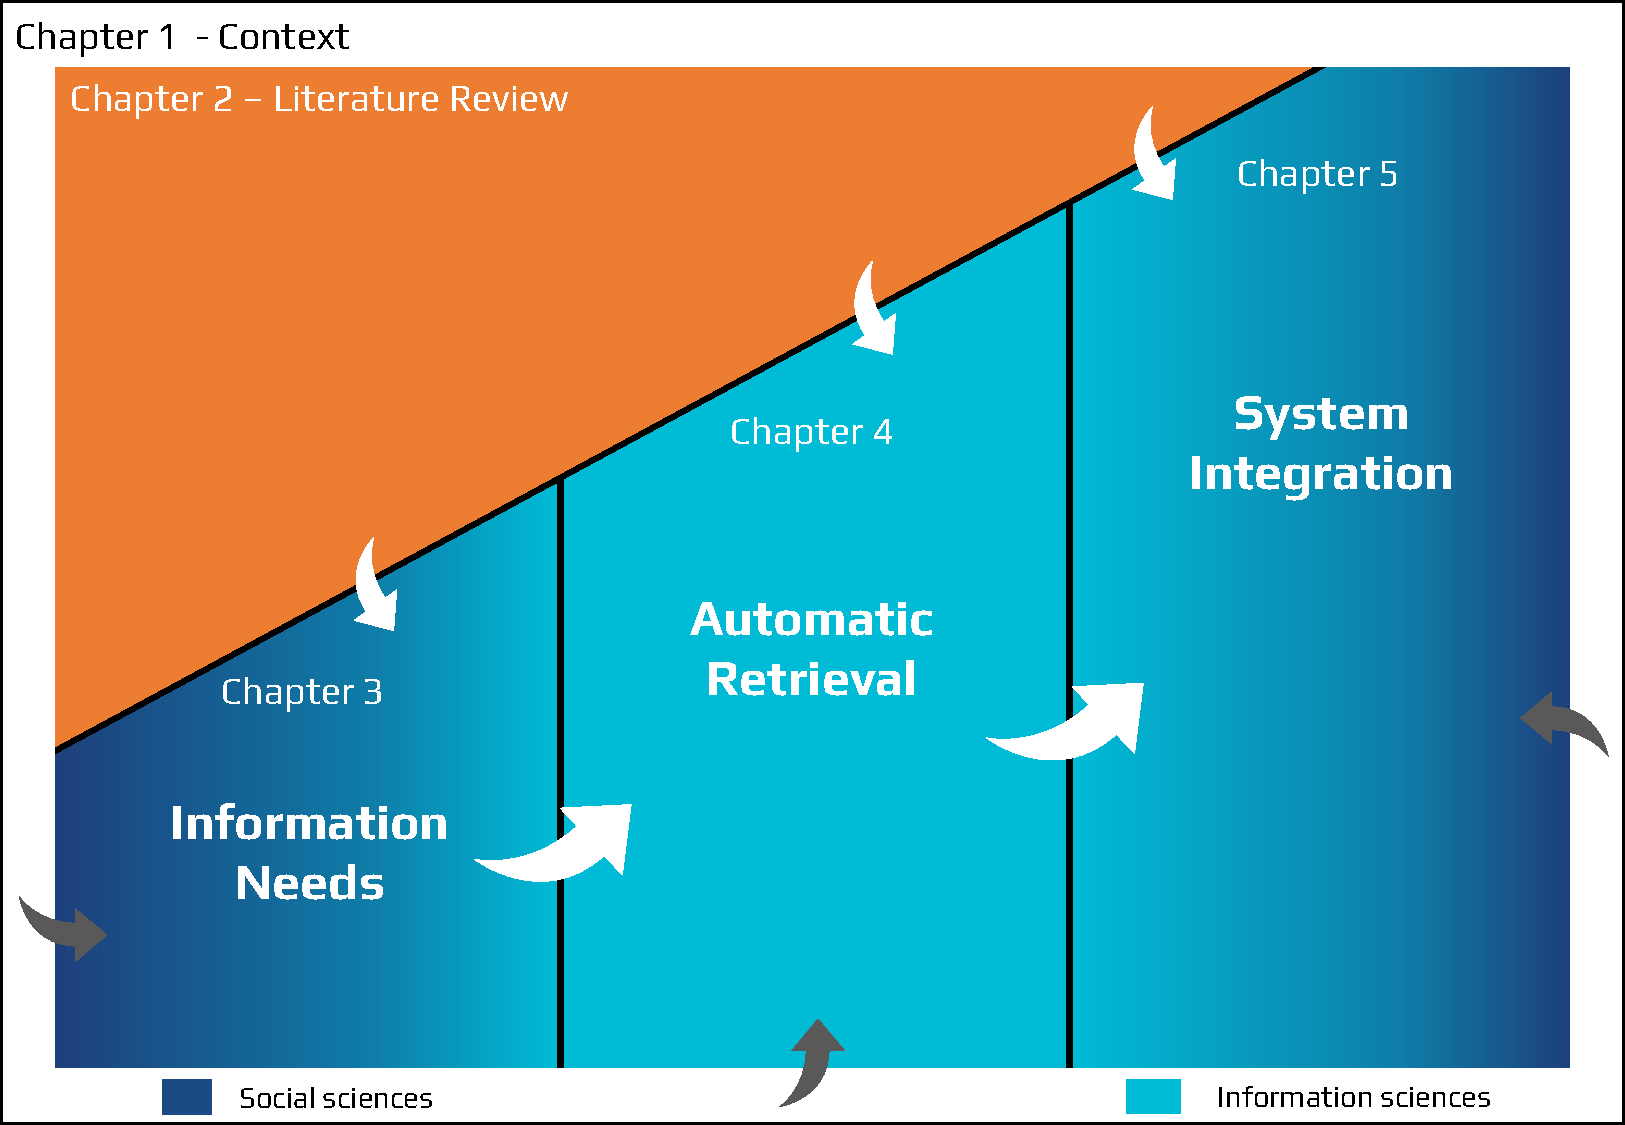
\includegraphics[width=0.92\textwidth,keepaspectratio]{figures/chap-0/big-picture.pdf}
    \caption{Overall organisation of the document. The arrows indicate the contribution of each part on the others.}
    \label{introduction:big-picture}
\end{figure}

%%% Local Variables:
%%% mode: latex
%%% TeX-master: "../ma-these"
%%% End:
